\documentclass[a4paper,12pt]{article}

\usepackage{latexsym}
\usepackage{amsfonts}
\usepackage{amsmath}
\usepackage{amsthm}
\usepackage{amssymb}
\usepackage{bbm}
\usepackage{graphicx}
\usepackage[normalem]{ulem}

\usepackage{hyperref}
\hypersetup{colorlinks=true,linkcolor=blue}

\usepackage{textcomp}
\usepackage{lmodern}
\usepackage[a4paper]{geometry}	
\usepackage[utf8]{inputenc}
\usepackage[T1]{fontenc}

\newcounter{numtho}
\newtheorem{remark}[numtho]{Remark}
\newcommand{\info}[1]{\texttt{#1}}

\begin{document}

\title{Lora's user manual}
\author{Laurent Claessens}
\maketitle

Lora is a backup program and a small Git remainder utility\footnote{Did you committed all your changes today ?}.

\begin{center}
    {\bf Warning}
\end{center}
This is a \emph{libre} software\footnote{In the sense of the GPL : no warranty, etc.} manipulating your precious data. If you use it, I consider you as a consenting adult.

\tableofcontents

%+++++++++++++++++++++++++++++++++++++++++++++++++++++++++++++++++++++++++++++++++++++++++++++++++++++++++++++++++++++++++++ 
\section{Compilation and installation}
%+++++++++++++++++++++++++++++++++++++++++++++++++++++++++++++++++++++++++++++++++++++++++++++++++++++++++++++++++++++++++++

The first step is to download the whole on \href{ https://github.com/LaurentClaessens/lora  }{ github } with
\begin{verbatim}
    git clone https://github.com/LaurentClaessens/lora
\end{verbatim}
You compile this documentation with
\begin{verbatim}
    pdflatex manual.tex
    pdflatex relazione.tex
\end{verbatim}

%--------------------------------------------------------------------------------------------------------------------------- 
\subsection{The manual way}
%---------------------------------------------------------------------------------------------------------------------------

\begin{enumerate}
    \item
        Create your \info{lora.cfg} looking at \info{example.cfg} for example and explanations.
    \item
        Modify the path of \info{BOOST\_THREAD\_LIB} in \info{makefile}.
    \item
        Modify the path of \info{MOC\_BIN} in \info{makefile}.
    \item
        Test with \info{./tests.sh} This should compile everything and launch a small testing program\footnote{This step does not work on the ``project'' branch. In other words, if you are reading this as professor at unipd, this will not work. The reason is that the tests use \info{std::function<void()>} from C++11 }.
    \item
        Compile : \info{make all}
    \item
        Launch Lora with \info{./lora}
\end{enumerate}

%--------------------------------------------------------------------------------------------------------------------------- 
\subsection{The graphical way}
%---------------------------------------------------------------------------------------------------------------------------

There is a graphical program that serves to make your configuration. 

%///////////////////////////////////////////////////////////////////////////////////////////////////////////////////////////
\subsubsection{Compile the installation program}
%///////////////////////////////////////////////////////////////////////////////////////////////////////////////////////////

\begin{enumerate}
    \item
        Compile the installation program :
        \begin{center}
            \info{make installation}
        \end{center}
    \item
        Launch the installation program :
        \begin{center}
            \info{./installation}
        \end{center}
\end{enumerate}

%///////////////////////////////////////////////////////////////////////////////////////////////////////////////////////////
\subsubsection{The backup tab}
%///////////////////////////////////////////////////////////////////////////////////////////////////////////////////////////

Here it is :

\begin{center}
    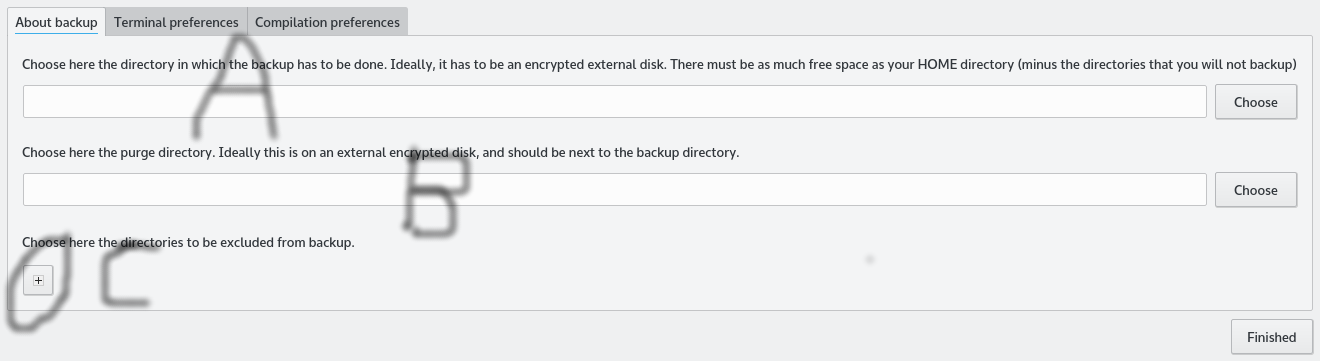
\includegraphics[width=\linewidth]{backup_tab.png}
\end{center}

\begin{enumerate}
    \item
        The backup directory (A) is the directory in which you want your \info{\$HOME} to be copied. Typically it will be something like
        \begin{center}
            \info{/mnt/backup\_partition/backup.lora}
        \end{center}
        where \info{/mnt/backup\_partition} is the mount point of an encrypted partition on an external drive.
    \item
        The purge directory (B) is the directory in which modified and removed files will be copied (from the backup directory) before to the respectively copied from the home to the backup and removed from the backup directory. The main user case is «I accidentally deleted a file, I perform the backup (thus the file is deleted from the backup) and \emph{then} I note that the file was removed.»  In this case, the removed file (in the version that was available in the backup) can be retrieved in the purge directory.

        Typically it will be something like
        \begin{center}
            \info{/mnt/backup\_partition/purge.lora}
        \end{center}

        Note that there are no automatic process removing the files from the purge directory. The size is then always increasing and you should remove very old subdirectory by hand.

        If you are using a program like Thunderbird, I let you know that it will \href{ http://xkcd.com/725/ }{ literally} produce \href{ https://fr.wikipedia.org/wiki/Gibioctet }{gibis} of data in the purge directory each day.
    \item
        The excluded directories (C) are what they seem to be : they will be excluded from the backup. You can as example not backup the directory in which you save the \info{iso} files of your preferred Linux distribution. Press the 
\includegraphics{plus.png} button to add an excluded directory.
\end{enumerate}

%///////////////////////////////////////////////////////////////////////////////////////////////////////////////////////////
\subsubsection{The terminal tab}
%///////////////////////////////////////////////////////////////////////////////////////////////////////////////////////////

You can skip this if you don't use git. 

The ``Terminal tab'' allows you to determine what kind of terminal and editor you prefer\footnote{Serious people use \sout{gedit} vim or \sout{notepad}emacs inside \sout{konsole}\,\sout{command.com}terminology.}.
Here is the tab :

\begin{center}
    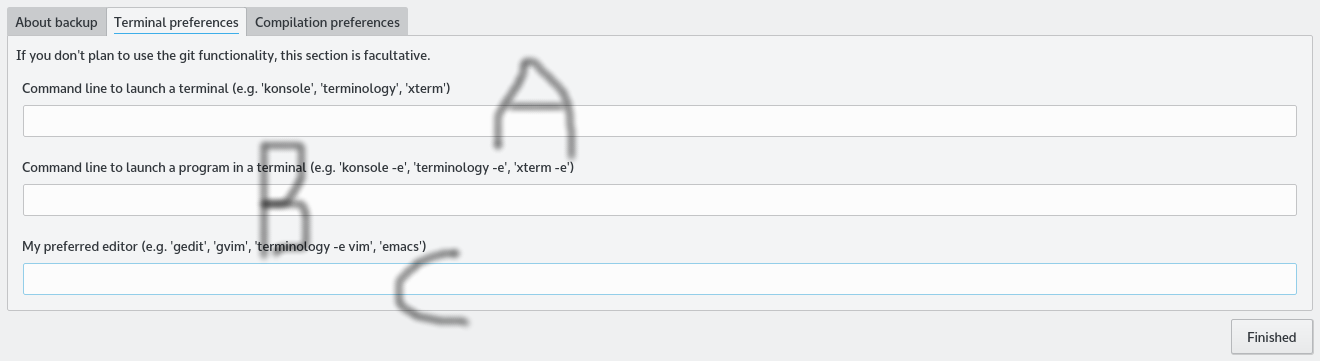
\includegraphics[width=\linewidth]{terminal_tab.png}
\end{center}
\begin{enumerate}
    \item
        The line (A) ask you the command line that launch your favorite terminal. This will be \info{konsole}, \info{terminology}, \info{xterm} or something like that. This is used when clicking on ``Open a terminal here''.
    \item
        The line (B) ask you how to launch a process in your terminal. The point is that \info{git diff} has to be launched in a terminal in order to take into account you git preferences\footnote{By the way, you should add \info{quotepath=false} in your \info{.gitconfig} file.}.
    \item
        The line (C) ask you your editor. This is used when clicking on ``Edit .gitignore''. If your favorite editor works in a terminal, you need to ask for opening a new terminal, e.g. \info{konsole -e vim} instead of simply \info{vim}.
\end{enumerate}

%///////////////////////////////////////////////////////////////////////////////////////////////////////////////////////////
\subsubsection{The compilation tab}
%///////////////////////////////////////////////////////////////////////////////////////////////////////////////////////////

If making
\begin{center}
    \info{make all}
\end{center}
works on the first strike, you can ignore this step.

Here is the compilation tab :
\begin{center}
    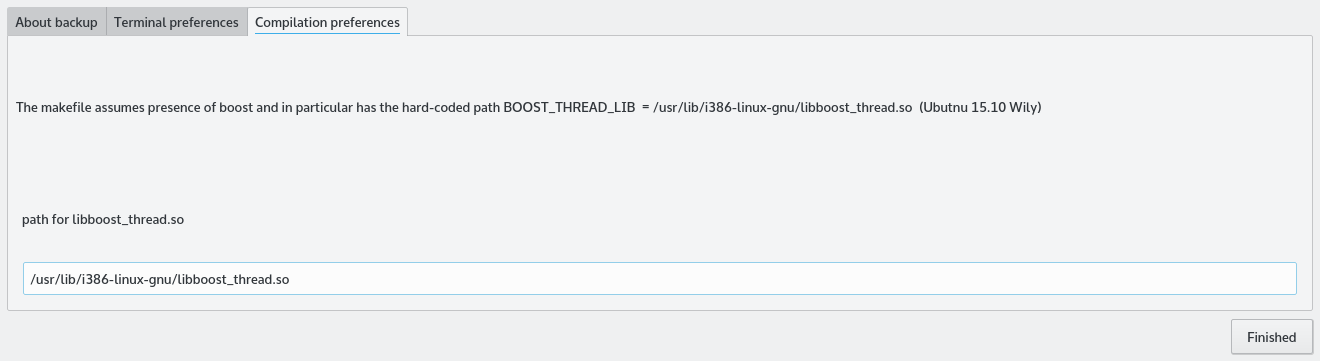
\includegraphics[width=\linewidth]{compilation_tab.png}
\end{center}

This asks you the path of the file \info{libboost\_thread.so} and the \info{moc} program that is mandatory for the compilation of Lora.

The file \info{auto\_makefile} is created and you will be able to compile Lora with this makefile.

%--------------------------------------------------------------------------------------------------------------------------- 
\subsection{Compilation}
%---------------------------------------------------------------------------------------------------------------------------

You need Boost to be installed somewhere on your system\footnote{On my Ubuntu, I do \info{apt install libboost-all-dev  libboost1.58-all-dev }}. The path to the file \info{libboost\_thread.so} has to be correct in the makefile (edit it if you are unsure).

For compiling everything you simply type
\begin{center}
    \info{make all}
\end{center}

%+++++++++++++++++++++++++++++++++++++++++++++++++++++++++++++++++++++++++++++++++++++++++++++++++++++++++++++++++++++++++++ 
\section{Testing}
%+++++++++++++++++++++++++++++++++++++++++++++++++++++++++++++++++++++++++++++++++++++++++++++++++++++++++++++++++++++++++++

You can test Lora by
\begin{center}
    \info{./tests.sh}
\end{center}
This will test some functionalities (for regressions) and allow you to see a Git window. If something gets wrong, send me an email at \info{laurent.claesens@studenti.unipd.it}

%+++++++++++++++++++++++++++++++++++++++++++++++++++++++++++++++++++++++++++++++++++++++++++++++++++++++++++++++++++++++++++ 
\section{Playing with Lora}
%+++++++++++++++++++++++++++++++++++++++++++++++++++++++++++++++++++++++++++++++++++++++++++++++++++++++++++++++++++++++++++

%--------------------------------------------------------------------------------------------------------------------------- 
\subsection{Backup}
%---------------------------------------------------------------------------------------------------------------------------

Launch
\begin{center}
      \info{./lora --configuration=<configuration\_filename>  <starting\_path>  }
\end{center}

\begin{description}
    \item[Configuration] Default is \info{lora.cfg}. The filename in which Lora has to read your configuration.
    \item[Starting path] Default is \info{\$HOME}. Giving the argument overrides the starting path written in the configuration file. If you want to backup only a part of your home because you only have \( 5\) minutes to shut down your computer.
\end{description}
Most of time you only have to launch \info{./lora} with no arguments.

Lora will loop over your home directory (or \info{starting\_path} if given in command line or in the configuration file) and compare\footnote{Files are different if they size differ or if they \info{last\_write\_time} attribute differ.} each file with the corresponding one in your backup directory. 
\begin{enumerate}
    \item
        If \info{<home>/foo/bar.txt} differs from \info{<backup>/foo/bar.txt}. 
        \begin{itemize}
            \item Move \info{<backup>/foo/bar.txt} to \info{<purge>/foo/bar.txt} Thus you will never loose data\footnote{Never in the sense of the GPL no warranty stuff\ldots}. In this sense, Lora is more than a \emph{synchronizing} program. It synchronizes and keeps the old data.
            \item Copy \info{<home>/foo/bar.txt} to \info{<backup>/foo/bar.txt}
        \end{itemize}
        If \info{<home>/foo/bar.txt} exists and \info{<backup>/foo/bar.txt} does not exist.
        \begin{itemize}
            \item Copy.
        \end{itemize}
\end{enumerate}

%--------------------------------------------------------------------------------------------------------------------------- 
\subsection{Purge}
%---------------------------------------------------------------------------------------------------------------------------

When the backup is finished, Lora will loop over your \info{<backup>} directory.

If \info{<backup>/foo/bar.txt} exists and \info{<home>/foo/bar.txt} does not exist, we deduce that you removed your file.
\begin{itemize}
    \item 
        Move \info{<backup>/foo/bar.txt} to \info{<purge>/foo/bar.txt}.
\end{itemize}
Note. The purge directory here is not exactly the same as the previous one. In fact each time you launch Lora, a new directory is created :
\begin{center}
    \info{<purge>/<date>/<hour-minutes>}
\end{center}
Inside that directory, Lora creates two directories : \info{modified} and \info{removed} which contain the files that were respectively seen to be modified and removed.

A general concept of Lora is that your data is more precious than your disk space and than everything\footnote{Better to crash than to manage a borderline situation.}. If you understand well the backup/purge concept, you can imagine the extreme disk space waste when you just rename, say your music directory.

%--------------------------------------------------------------------------------------------------------------------------- 
\subsection{The Git helper}
%---------------------------------------------------------------------------------------------------------------------------

Since Lora loops over the whole \info{\$HOME}, it also takes time to check for each directory if it is a git repository (has non trivial .git subdirectory) and if this repository is clean\footnote{I personally gitted directories like \info{.config} and \info{.kde}, so I am not always conscient that a git repository have been modified.}.

A list of directories that are not clean git repository (untracked or modified files) is displayed. Clicking on one of them opens a dialog window that helps you to manage the situation.

Here is a window example :

\begin{center}
    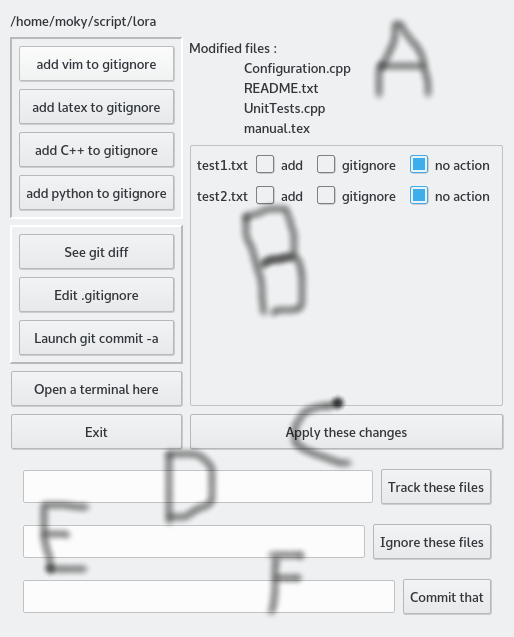
\includegraphics[width=\linewidth]{git_helper.png}
\end{center}

\begin{enumerate}
    \item
        A list of modified files (A).
    \item
        A list of untracked files (B). For each you can choice to track it (add) or ignore it (add to \info{.gitignore}). When clicking on ``Apply these changes'' (C), Lora does \info{git add} for the files you checked ``add'' and appends to \info{.gitignore} the names that you checked as ``gitignore''.
    \item
        The ``Track these files'' line (D). Lora will perform \info{git add} with the given argument (like \info{*.cpp}, \info{*.tex}).
    \item
        The ``Ignore these files'' line (E). Lora will append the files given in argument into \info{.gitignore} (like \info{*.tmp}, \info{*.eps}).
    \item
        The ``Commit that'' line (F) performs \info{git commit --message=} with the given message.
\end{enumerate}


\begin{description} 
    \item[Add <this> to gitignore] Click there is this repository is of <this> type and Lora will add corresponding files to \info{.gitignore}. Example : with ``add latex to gitignore'', it will add \info{*.aux}, \info{*.toc}, etc.
    \item[See git diff]
        Open a terminal and launch \info{git diff} inside.  

        The behaviour of all the git part could depend on your local git configuration. As an example, the button \emph{See git diff} will open a terminal and launch \info{git diff} inside. If you have configured git in such a way that \info{git diff} only prints the diff, then the terminal will be immediately closed. Thus if you want to take benefit of this functionality on Lora you should add something like

\begin{verbatim}
[diff]
    external =  vimdiff
\end{verbatim}
in your \info{.gitconfig}.
    \item[Edit .gitignore] Open \info{.gitignore} in your preferred editor.
    \item[Launch git commit -a] Open a terminal and launches \info{git commit -a} inside.
    \item[Open a terminal here] Does what you think it does.
    \item[Exit] Does what you think it does.
\end{description}

%+++++++++++++++++++++++++++++++++++++++++++++++++++++++++++++++++++++++++++++++++++++++++++++++++++++++++++++++++++++++++++ 
\section{Known issues}
%+++++++++++++++++++++++++++++++++++++++++++++++++++++++++++++++++++++++++++++++++++++++++++++++++++++++++++++++++++++++++++

There are still several cases in which Lora crashes. The general ideology is that your data is precious and \emph{you} should manage border line cases. Anyway, some crashes are known and some improvement in their managing have to be done in Lora.
\begin{enumerate}
    \item
        Crash when one has not the read permission in a file. But really, do you have a file in \emph{your} home on which you don't even have the reading permission ? Sadly, the answer could be \emph{yes}.
    \item
        Some filenames seem to pose problems. As an example : \url{~/.local/share/gvfs-metadata/network:} provokes a crash ``invalid argument'' on Boost's filesystem \info{copy\_file}. Some investigations show that this could be related to the colon in the filename.
    \item
       Deleting a file during the backup process could lead to a crash ``file not found''. Multithreading make this one not easily reproducible.
    \item
        When the \info{last\_write\_time} attribute of a file in the backup is more recent than the one in the home, Lora crashes. Did you got back an old version of a file ? I got that crash in the following way :
        \begin{itemize}
            \item clone a git repository,
            \item modify a file,
            \item backup with Lora,
            \item remove the directory and re-clone it. Then the ``new'' file has the last write time attribute of the ``origin'' one while the file in the backup as the time of \emph{your} modification.
            \item backup with Lora will crash with an useful error message.
        \end{itemize}
        By the way, here the crash has to be seen as a feature more than a bug because you \emph{really} lost data and you should \emph{really} worry.
\end{enumerate}

\end{document}

